\documentclass[11pt, twoside]{book}
\usepackage[full]{leadsheets}
\usepackage[a4paper,  hmargin=1.5cm, vmargin=3cm, head=14pt, foot=50pt]{geometry}
\usepackage{multicol}
\usepackage[polish]{babel}
\usepackage{array}
\usepackage{graphicx}
\usepackage{hyperref}
\usepackage{tocloft}
\usepackage[toc]{multitoc}
\usepackage{fancyhdr}
\usepackage{tikzpagenodes}
\usepackage{titlesec}
\usepackage{tabularx}
\usepackage{adjustbox}
\usepackage{tipa}
\usepackage{ifxetex}
\usepackage[%
    left = \glqq,%
    right = \grqq,%
    leftsub = «,%
    rightsub = »%
]{dirtytalk}

\thispagestyle{empty}

\ifxetex%
    \usepackage{substitutefont}
    \substitutefont{T3}{\rmdefault}{cmr}
\fi

%\usepackage[default]{lato}
%\usepackage[T1]{fontenc}

\selectlanguage{polish}
\DeclareTranslation{Polish}{leadsheets/chorus}{Ref.}
\DeclareTranslation{Polish}{leadsheets/interlude}{Przej.}
\DeclareTranslation{Polish}{leadsheets/lyrics}{tekst}
\DeclareTranslation{Polish}{leadsheets/verse}{Zwr.}
%\DeclareTranslation{Polish}{leadsheets/capo}{Kapo}
\DeclareTranslation{Polish}{leadsheets/fret}{próg}

% Tytuł spisu treści
\addto\captionspolish{\renewcommand*\contentsname{Jakieś piosenki}}

\definesongtitletemplate{custom}{%
    \let\clearpage\relax
    \ifsongmeasuring%
        {\section*}
        {\section}%
        {\songproperty{title}}%
    \begingroup\footnotesize
        \begin{tabular}{%
                @{}
                >{\raggedright\arraybackslash}p{.5\linewidth}
                @{}
                >{\raggedleft\arraybackslash}p{.5\linewidth}
                @{}
            }
            \ifsongproperty{music}{%
                Muzyka: \songproperty{music} \\%
                }{}%
            \ifsongproperty{lyrics}{%
                Tekst: \songproperty{lyrics} \\%
                }{}%
            \ifsongproperty{interpret}{%
                Interpretacja: \songproperty{interpret} \\%
                }{}%
            \ifsongproperty{capo}{%
                & \capo{} \\%
                }{}%
        \end{tabular}%
        \par
    \endgroup
}

\setleadsheets{%
    title-template = custom,
    verse/numbered,
    remember-chords=false,
    align-chords={l},
    capo-nr-format=arabic,
    bar-shortcuts
}
\setchords{%
    minor={lowercase},
    input-notation=german,
    output-notation=german
}

\renewcommand{\chaptermark}[1]{\markboth{#1}{}}

\fancypagestyle{plain}{%
    \fancyhf{}
    \fancyhead[L]{Jakieś piosenki}
    \fancyfoot[LE,RO]{\Large\thepage}
}
\fancypagestyle{szanty}{%
    \pagestyle{plain}
    %\fancyhf{}
    %\fancyhead[L]{Jakieś piosenki}
    \fancyhead[R]{Szanty}
    %\fancyfoot[LE,RO]{\Large\thepage}
    \fancyfoot[LO]{
\includegraphics[height=45pt]{images/kolo.png}}
    \fancyfoot[RE]{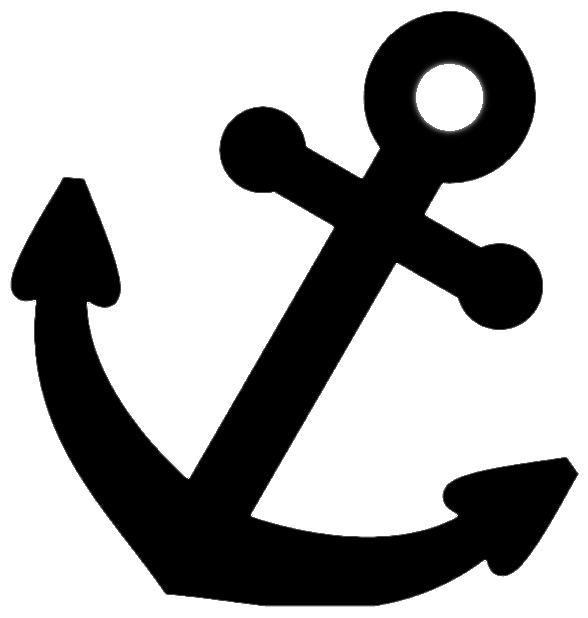
\includegraphics[height=45pt]{images/kotwica.png}}
}
\fancypagestyle{poezja}{%
    \pagestyle{plain}
    \fancyhead[R]{Poezja śpiewana}
    \fancyfoot[LO]{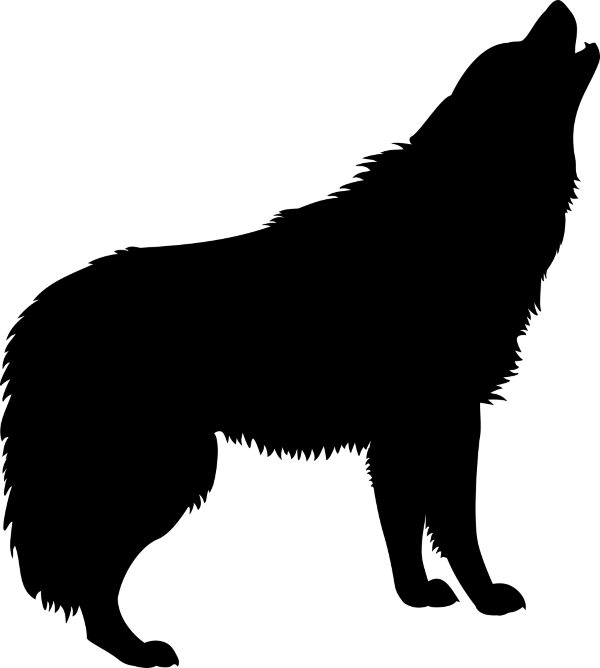
\includegraphics[height=45pt]{images/wilk.png}}
    \fancyfoot[RE]{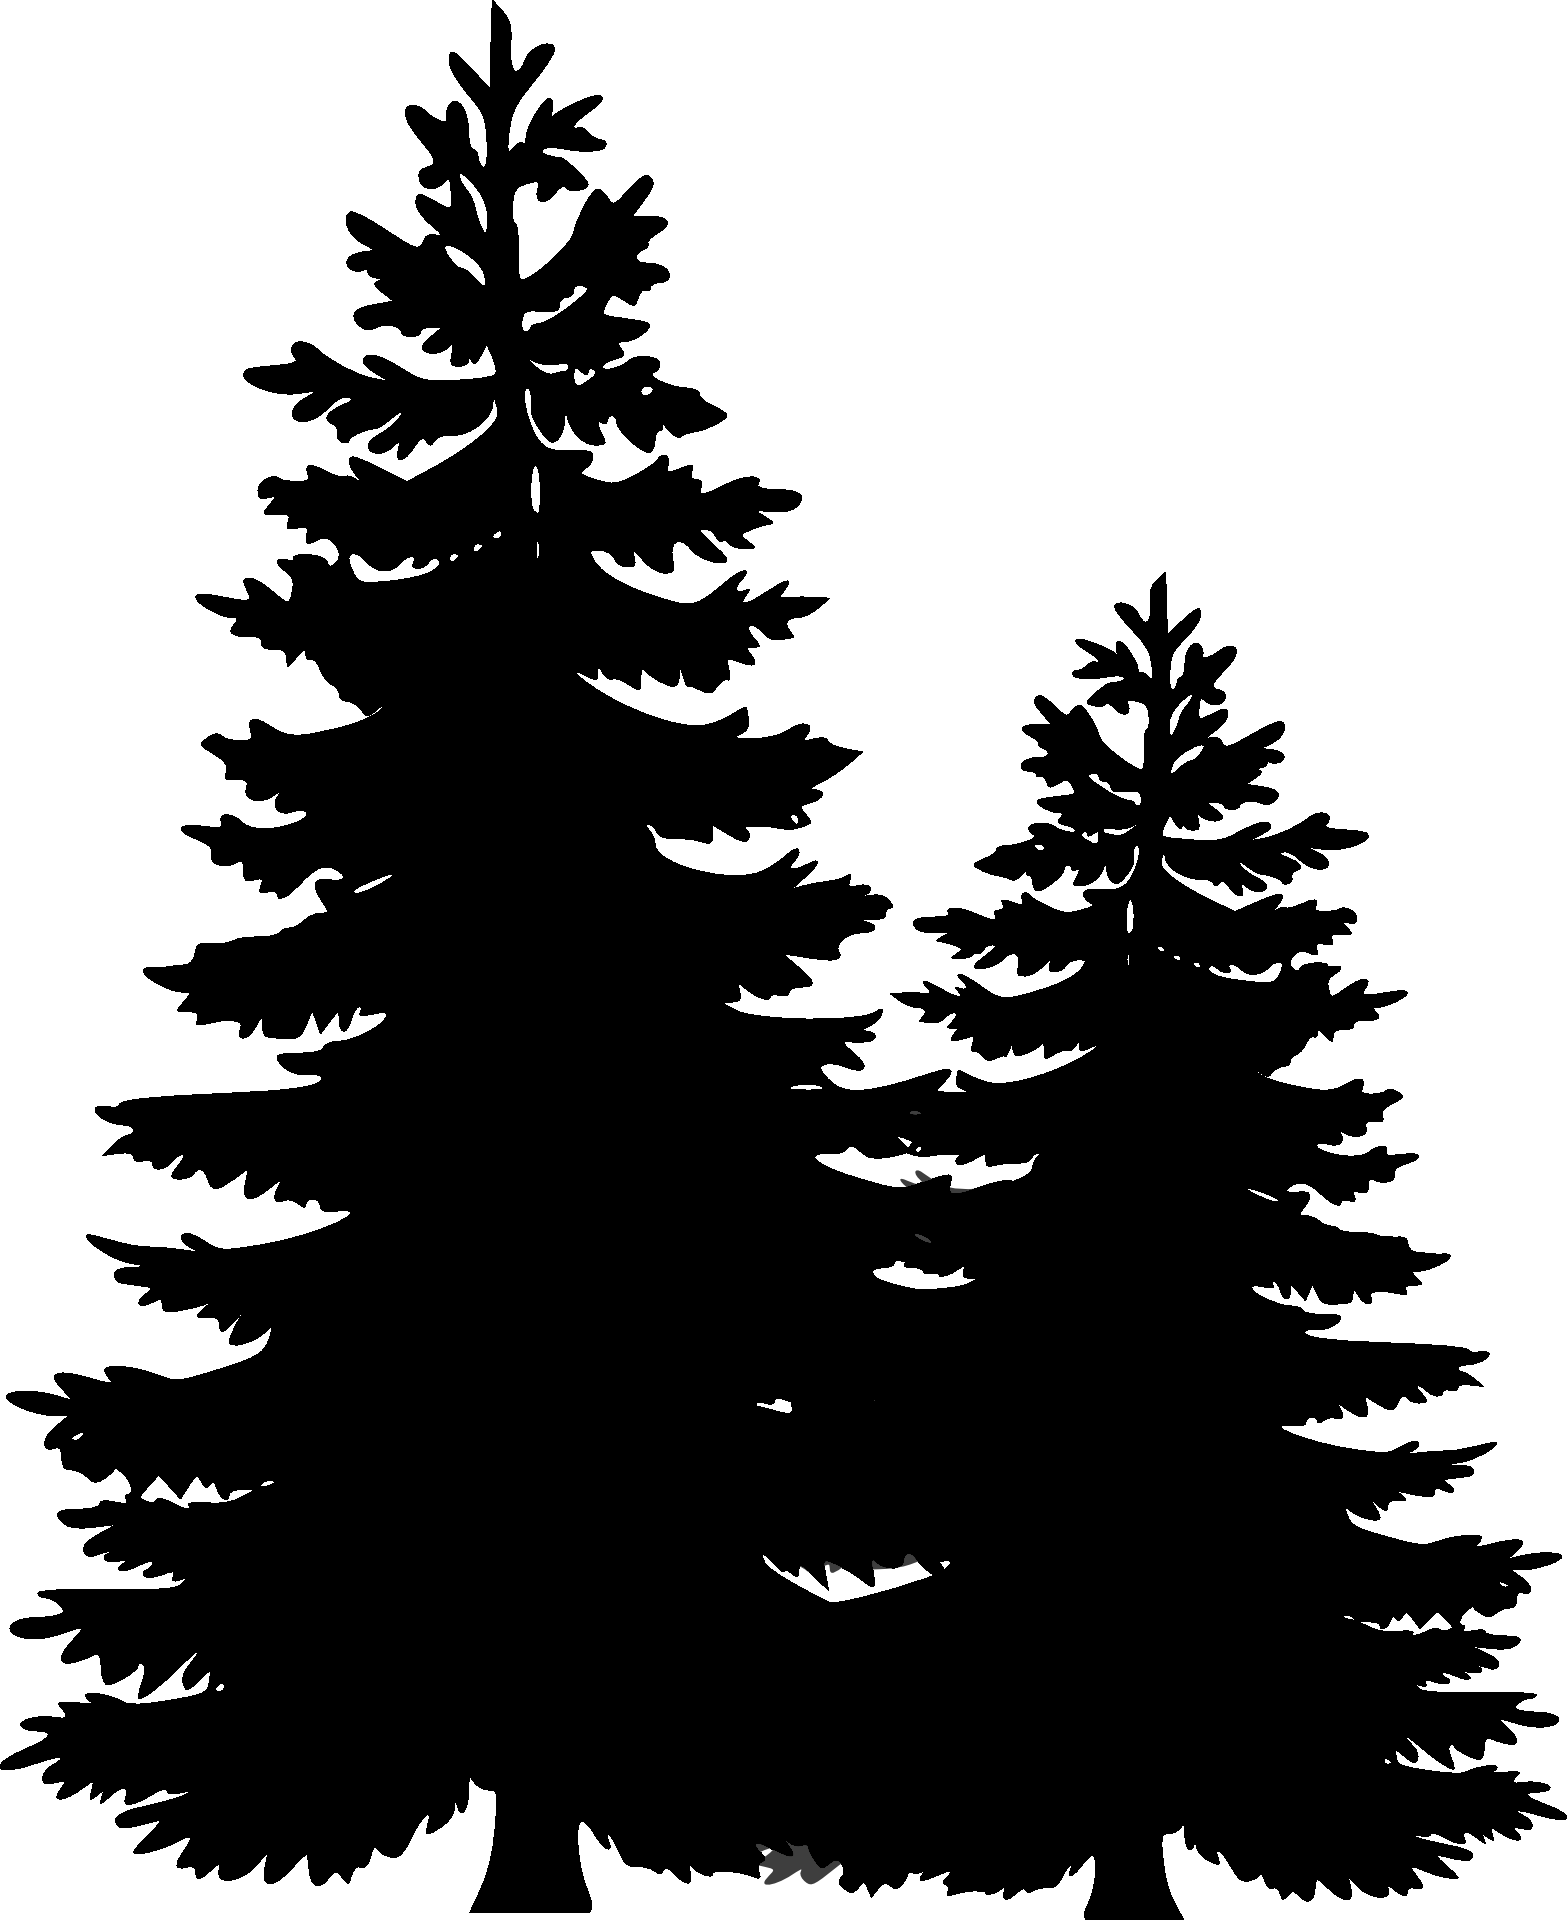
\includegraphics[height=45pt]{images/drzewa.png}}
}
\fancypagestyle{pop}{%
    \pagestyle{plain}
    \fancyhead[R]{Pop}
    \fancyfoot[LO]{
\includegraphics[height=45pt]{images/gwiazdy.png}}
    \fancyfoot[RE]{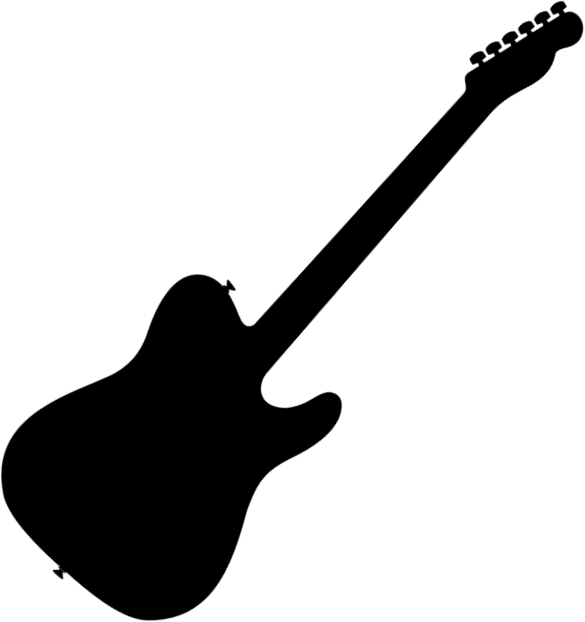
\includegraphics[height=45pt]{images/gitara.png}}
}

\renewcommand{\cftdot}{\ensuremath{\sim}}
\renewcommand{\cftsecleader}{\cftdotfill{\cftdotsep}}

% Usunięcie numeru rozdziału sprzed numeru sekcji
%\renewcommand{\thesection}{\arabic{section}}

\titleformat{\chapter}[block]{\centering\vspace{6cm}}{}{0pt}{\Huge\bfseries}

\newversetype{riff}[name={Riff}, numbered=false, named=true]

\counterwithin*{footnote}{section}


\begin{document}

\begin{titlepage}
    \begin{center}
        \vspace*{5cm}
        
        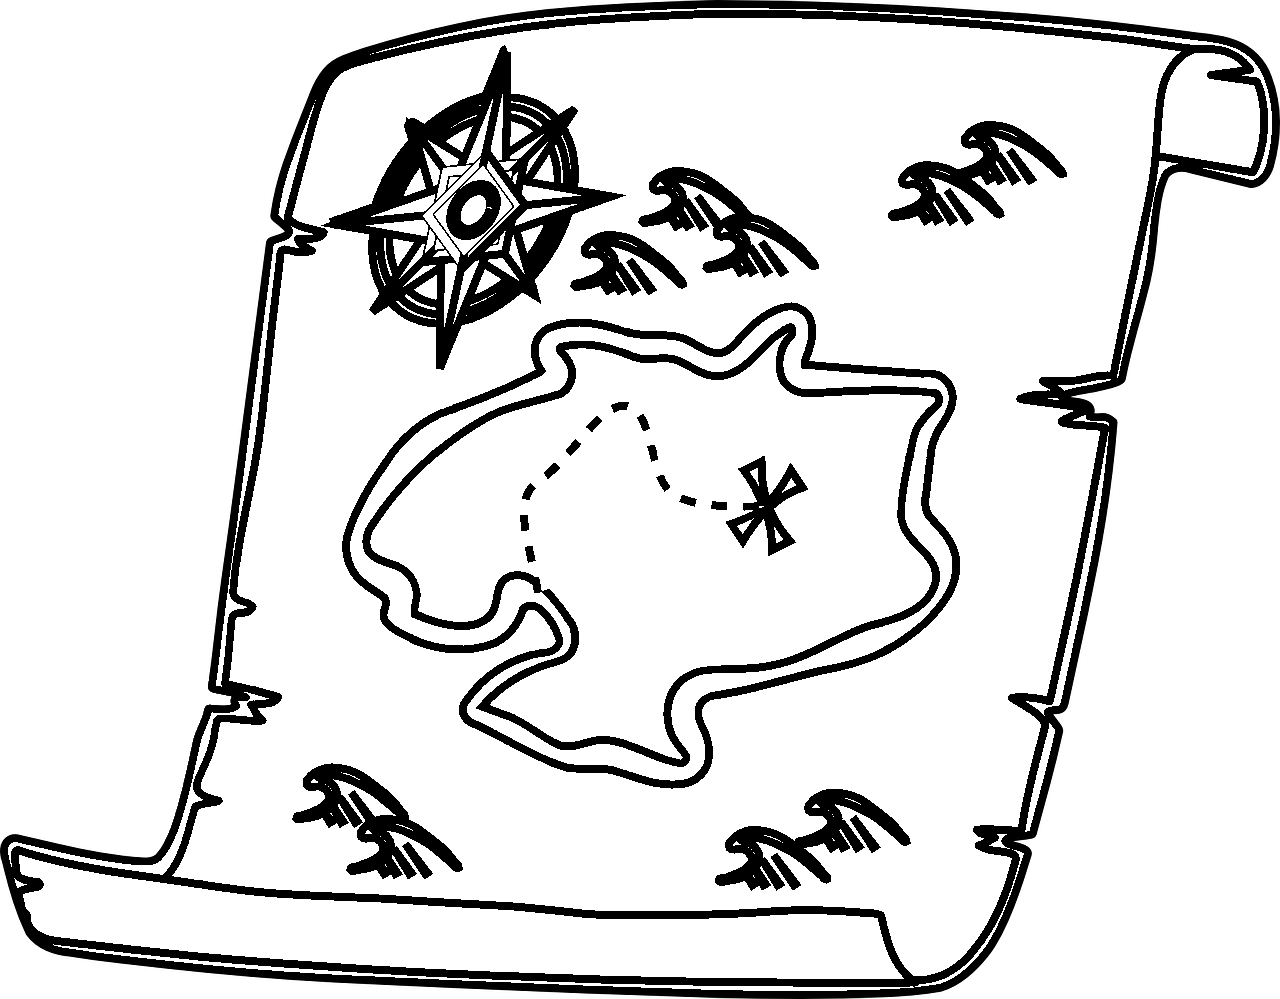
\includegraphics[height=8cm]{images/front-obrazek-aneks.png}

        \vspace{1.5cm}

        \Huge\textbf{Jakieś piosenki}
        
        \vspace{0.5cm}
        \Large Aneks dla niegrających na gitarze \\
        \LARGE Wydanie pierwsze
        
        \vfill

        \Large
        Wydawnictwo Kis Inkris \\
        Warszawa, 2021

        %\vspace{0.5cm}

        %\footnotesize
        %https://github.com/dzierzanowski/spiewnik-szant

        %\begin{tikzpicture}[remember picture,overlay,shift={(current page.south east)}]
        %    \node[anchor=south east,xshift=0cm,yshift=0cm]{
\includegraphics[width=3.5cm]{images/qr.png}};
        %\end{tikzpicture}
    \end{center}
\end{titlepage}

\tableofcontents
\vfill
\renewcommand{\tabularxcolumn}[1]{>{\small}b{#1}}
\begin{adjustbox}{width={\textwidth}, keepaspectratio}  % Korekta sumarycznej szerokości creditsów i kodu QR
\begin{tabularx}{\textwidth}{%
        @{}
        >{\raggedright\arraybackslash}X
        @{}
        >{\raggedleft\arraybackslash}X
    }
    \footnotesize
    Kamil Dzierżanowski --- opracowanie, skład, korekta

    Paweł Kulig --- opracowanie

    \medskip

    https://github.com/dzierzanowski/spiewnik-szant

    &

    Pobierz śpiewnik online:

    
\includegraphics[width=3cm]{images/qr.png}
\end{tabularx}
\end{adjustbox}

\chapter{Szanty}
\begin{center}
    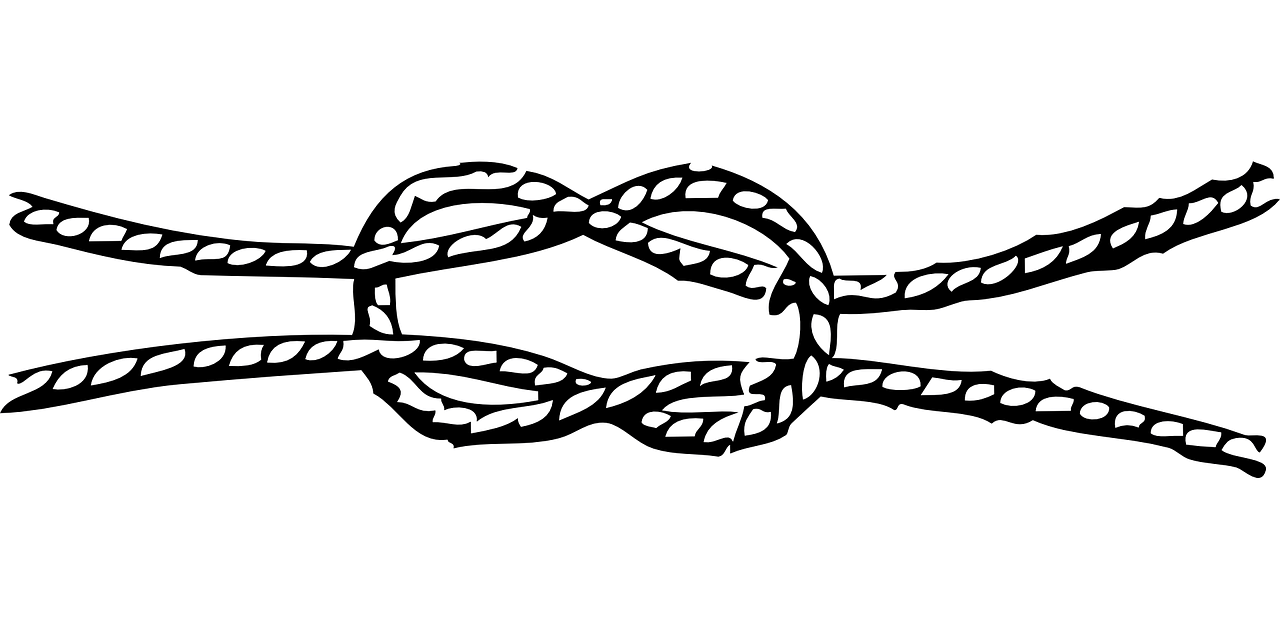
\includegraphics[width=0.5\textwidth]{images/wezel.png}
\end{center}
\pagestyle{szanty}
\newpage
\begin{song}{title={Press gang (Branka)}, music={Cztery Refy}}
    \begin{center}
        \includegraphics[width=\textwidth]{songs-alt/cztery\string_refy-press\string_gang.png}
    \end{center}
\begin{multicols}{2}
    \begin{verse}
        W dół od rzeki, poprzez London Street \\
        Psów królewskich oddział zwarty szedł \\
        Ojczyźnie trzeba dziś świeżej krwi \\
        Marynarzy floty wojennej
    \end{verse}
    \begin{verse}
        A że byłem wtedy silny chłop\\
        W tłumie złowił mnie sierżanta wzrok \\
        W kajdanach z bramy wywlekli mnie \\
        Marynarza floty wojennej
    \end{verse}
    \begin{verse}
        Jak o prawa upominać się \\
        Na gretingu nauczyli mnie \\
        Niejeden krwią wtedy spłynął grzbiet \\
        Marynarza floty wojennej
    \end{verse}
    \begin{verse}
        Nikt nie zliczy ile krwi i łez \\
        Wsiąkło w pokład, gdy się zaczął rejs \\
        Dla chwały twej, słodki kraju mój \\
        Marynarzy floty wojennej
    \end{verse}
    \begin{verse}
        Hen, za rufą miły został dom \\
        Jesteś tylko parą silnych rąk \\
        Dowódca tu twoim bogiem jest \\
        Marynarzu floty wojennej
    \end{verse}
    \begin{verse}
        Gdy łapaczy szyk formuje się \\
        W pierwszym rzędzie możesz ujrzeć mnie \\
        Kto stanie na mojej drodze dziś \\
        \textbf{Łup} stanowi floty wojennej
    \end{verse}
\end{multicols}
\end{song}

\newpage
\begin{song}{title={Few days}, music={Ryczące Dwudziestki}}
    \medskip
    \begin{adjustbox}{width={\textwidth}, keepaspectratio}
        \includegraphics[width=\textwidth]{songs-alt/ryczace\string_dwudziestki-few\string_days.png}
    \end{adjustbox}
    \begin{info}
        \textit{(beat jak w \say{We Will Rock You})}
    \end{info}
    \begin{multicols}{2}
    \begin{verse}
        O Panie, czemu w ziemi tkwię \\
		Hej raz, hej raz! \\
		I macham szuflą cały dzień? \\
		Hej, na morze czas! 
    \end{verse}
    \begin{chorus}
        Mogę kopać tu dalej \\
		Few days, few days \\
		Mogę kopać przez dni parę \\ 
		Ale wracać chcę  $\times 2$ 
    \end{chorus}
    \begin{verse}
        Tam każdy takie bajdy plótł \\
		Nie raz, nie raz \\
		Przekroczysz Jukon, złota w bród \\
		Hej, na morze czas! 
    \end{verse}
    \begin{chorus}
        Mogę kopać tu dalej\ldots $\times 2$ 
    \end{chorus}
    \begin{verse}
        Wykopię jeszcze parę dziur \\
		Hej raz, hej raz \\
		Wytoczę płonnej skały wór \\
		Hej, na morze czas!
    \end{verse}
    \begin{chorus}
        Mogę kopać tu dalej\ldots $\times 2$ 
    \end{chorus}
    \begin{verse}
        Za żonę tu łopatę mam \\
		Już dość, już dość \\
		A zysk, że jej uzywam sam \\
		Hej, na morze czas!
    \end{verse}
    \begin{chorus}
        Mogę kopać tu dalej\ldots $\times 2$ 
    \end{chorus}
    \begin{verse}
        O Panie nie jest to Twój raj \\
		O nie, o nie \\
		Nadzieję innym głupcom daj \\
		Ja na morze chcę!
    \end{verse}
    \begin{chorus}
        Chociaż już mi wystarczy \\
		Few days, few days \\
		Dam Ci jeszcze jedną szansę \\
		Ale wracać chcę $\times 2$ 
    \end{chorus}
    \end{multicols}
\end{song}



\chapter{Poezja śpiewana}
\begin{center}
    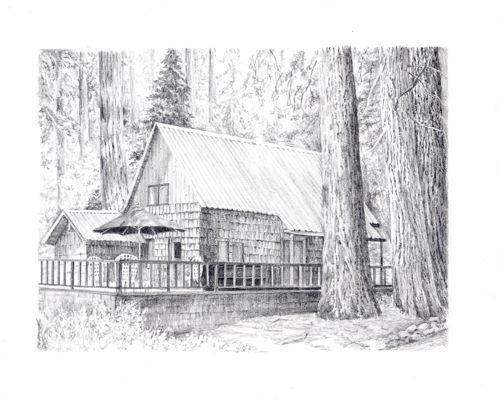
\includegraphics[width=0.5\textwidth]{images/chatka.jpg}
\end{center}
\pagestyle{poezja}

\chapter{Pop}
\begin{center}
    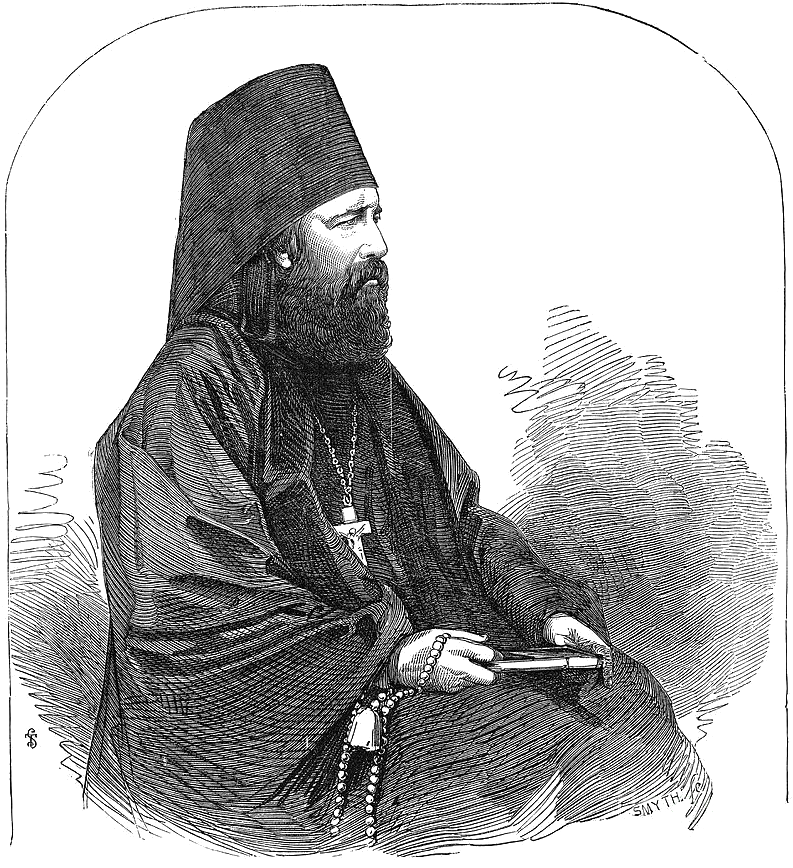
\includegraphics[width=0.4\textwidth]{images/pop.png}
\end{center}
\pagestyle{pop}

% Ostatnia strona parzysta pusta, żeby nie było tekstu na odwrocie
\clearpage{\mbox{}\pagestyle{empty}\cleardoublepage}

\end{document}
